\chapter{Introduction}%

Understanding the dynamics of ecological structures is very important in determining how climate, %CO\textsuperscript{2} emission, 
land cover %(water resources, desertification)
, fire hazards, and biodiversity evolve. Precision study of plant species is of high environmental and economical impacts which is only possible through geo-mapping the distribution of plant species abundances at ecological scale. Large scale study of ecological domains has been made possible through spaceborne or airborne campaigns utilizing remote sensing technologies such as \textit{(multi/hyper)-spectral} and \textit{LiDAR}. In this project we focus on airborne hyperspectral and LiDAR data. Each campaign covering tens of acres of land can generate terra-bytes of data depending on measurement resolution (large volume). On the other hand, apart from state-of-the-art machine learning algorithms, there is a great wealth of expert ecological knowledge covering a whole variety of domains (along with their in-ground associated data) that can be used to enhance species mapping that is not being used and is left for ecological scientists for manual interpretation (data variety). Furthermore, data is being generated at faster pace day after day as technology becomes more afordable. After satellite sensors, airborne sensors came into place and now as airborne is still costly there is a surge of interest towards more affordable drone campaigns \citep{zhou2009foreword}. So we are facing data being generated at unprecedented rates (data velocity). The final aspect is verasity: imperfect sensors, non-standardized measurements, atmosphere impacts (clouds, humidity, aerosols) and et cetera all create uncertainities that need to be accounted for. Velocity, verasity, volume, and variety are the four V's that indicate ecology is stepping into the realm of "big data"\citep{hampton2013big, soranno2014macrosystems}.

\section{Remote Sensing}

From an ecological point of view, there are two types of remote sensing approaches: active and passive. \textit{Passive} remote sensing uses sunlight as the source of energy and sensors captures the intensity of light being reflected from earth's surface. Light intensity measurements happens at various wavelengths; if a few (usually 3 to 10) relatively broad wavelength bands are captured it is called multi-spectral. If light intensity at dozens to hundreds of narrow band signals are collected it is called hyperspectral. \textit{Active} remote sensing on the other hand uses laser light emission as its source of energy and captures the intensity of returned signals. LiDAR is a popular active remote sensing technology. Below we explain each in more details:



\subsection{Hyperspectral}

\begin{figure}[b!]
  \centering
    \includegraphics[scale=0.22]{images/spectrometer.eps}
    \caption[Imaging spectrometer schematic diagram]{Schematic diagram of the basic elements of an imaging spectrometer where $\lambda$ is the wavelength \citep{smith2006introduction}.}
    \label{fig:Imaging spectrometer}
\end{figure}

Spectrometers measure the amount of light reflected from surface materials: An optical dispersing element (like a prism) refracts the received light into its constituent spectrums and the energy in each band range is measured by a separate detector. Bands can be as narrow as 0.01 $μm$ over a wide wavelength range of typically 0.4 to 2.5 $μm$. Figure~\ref{fig:Imaging spectrometer} shows the basic components of an imaging spectrometer.

Raw sensor readings (digital number) can be affected by light source conditions, sensor, atmosphere, and surface material. Raw data which is a unit-less light intensity measure is then calibrated into radiance which has a  physically meaningful unit through applying a gain and offset to the pixel values. It essentially means how much light the instrument ''sees'' from the object being observed. Some reference materials like a pure white or pure black sheets can be used in this process. After adjustments for sensor, atmospheric, and terrain effects are applied, pixel reflectance value is calculated which is the proportion of the radiation striking a surface to the radiation reflected off of it. Reflectance demonstrates light abroption features of the surface material and can be compared with field or laboratory reflectance spectra in order to recognize and map surface materials such as particular types of vegetation or diagnostic minerals associated with ore deposits. Reflectance varies with wavelength for most materials because energy at certain wavelengths is scattered or absorbed to different degrees \citep{smith2006introduction}. In this project we deal with reflectance values and refer the reader to \citep{varshney2004advanced} for more details on how to compute reflectance values.

\begin{figure}[t!]

  \centering
    \includegraphics[scale=0.45]{images/reflectanceAsIndicator.eps}
    \caption[Some reflectance examples]{Some reflectance examples as how reflectance of different material show different absroption features at differnet bands. \citep{smith2006introduction}.}
    \label{fig:Some reflectance examples}
\end{figure}

Figure~\ref{fig:Some reflectance examples} shows some example materials when observed through an spectrometer. In vegetations, chlorophyll and some leaf pigments show high absorptions in blue and red ranges and not so much in green; therefore our eyes see vegetation as green. We can see this as a small peak in green compared to other visible wavelength range. From red to near infrared there is a sharp rise known as \textit{red edge} up to a value of about 50\% for some plants. High values in the near-infrared region is mainly due to internal cellular structure of leaves which differs significantly across species but can also be different in a single specie due to plant stress. High reflectance in near-infrared can interact with other leaves in the canopy and therefore its sensor readings can be dependent on canopy structure as well. Beyond 1.3 $μm$ reflectance decreases with increasing wavelength, except for two pronounced water absorption bands near 1.4 and 1.9 $μm$. At the end of the growing season leaves lose water and chlorophyll. Near infrared reflectance decreases and red reflectance increases, creating the familiar yellow, brown, and red leaf colors of autumn \citep{smith2006introduction}.

\subsection{LiDAR}



\section{Data Variety}

As of 


%\begin{table}[h!]
%\caption{How to align decimals in a numerical column}\label{tb1}
%  \begin{tabular}{p{3 in} r@{.}l c}
% \hline
% Category & \multicolumn{2}{c}{Result}  & \hspace{2.2 in} \\
% \hline
%  first & 3&14159 & \hspace{2.2 in} \\
%  second & 16&2 & \hspace{2.2 in} \\
%  third & 123&456 & \hspace{2.2 in} \\
%  \hline
%  \end{tabular}
%\end{table}
%
%
%\begin{figure}[htbp]
%  \centering
%    
\includegraphics[width=3in, scale=0.5]{images/LaTeX2e_logo.eps}
%    \caption[\LaTeX 2\ensuremath{\epsilon} logo(resized for no reason)]{\LaTeX 2\ensuremath{\epsilon} logo, resized for no reason. This caption is being extended in order to test that it has the correct indentation.}
%\end{figure}





%
%\begin{figure}[htbp]
%  \begin{center}
%    \centering
%    \mbox{
%      \subfigure[]{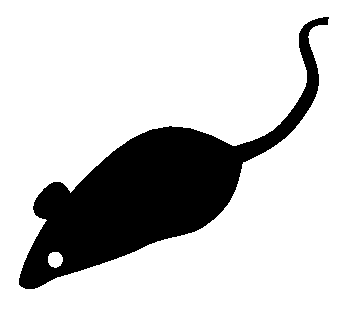
\epsfig{file=images/mouse.eps, scale=0.6}} \quad
%      \subfigure[]{\begin{turn}{20}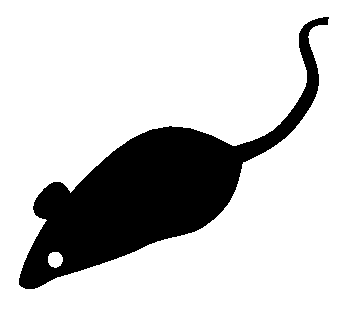
\epsfig{file=images/mouse.eps, scale=0.6}\end{turn}} \quad
%     }
%    \mbox{
%      \subfigure[]{\begin{turn}{-20}
\epsfig{file=images/cat.eps, scale=3}\end{turn}} \quad
%      \subfigure[]{\begin{turn}{-10}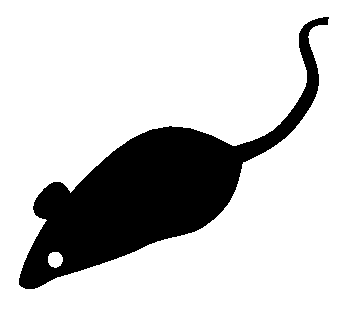
\epsfig{file=images/mouse.eps, scale=0.6}\end{turn}} \quad
%      }
%    \caption[Tom and Jerry]{Tom and Jerries? A) Mouse 1 B) mouse 2 C) Hungry Cat D) mouse 3}
%    \label{mice}
%  \end{center}
%\end{figure}

\subsection{Markov Logic Network}
Markov logic network is a probabilistic logic that applies the concept of Markov network to first order logic. For inference, instead of usning intractable algorithms of prolog or lisp, it uses MCMC sampling.

\section{Proposed Work}

\section{Proposal Structure}

% Mapping the spatial distribution of plant species in savannas provides insight into the roles of competition, fire, herbivory, soils and climate in maintaining the biodiversity of these ecosystems. 
 
% Savannas harbor spatially complex assemblages of vegetation that are mediated by an array of biotic and abiotic factors including plant competition, fire, herbivory, soils and climate [1–4]. Mapping the distribution of species abundances across spatial scales relevant to these processes is requisite to understanding their role in shaping and maintaining savanna biodiversity.
 
%%% Invasive plant species can change entire habitats by penetrating the native canopy and eventually replacing it [1]. At times, fundamental ecosystem processes such as nitrogen (N) cycling as well as disturbance regimes such as fire frequency are altered by the introduced species, resulting in a major change in biological diversity and ecosystem functioning [2].
 
% Effective management of introduced species starts with monitoring and mapping, which is a central component of the biological diversity protection programs of many government agencies and non- governmental organizations worldwide [3]. Remote detection and mapping of biodiversity and invasive species from airborne or spaceborne instruments is promising (review by [4]), but operational approaches are lacking because of our limited biophysical understanding of when remotely sensed signatures indicate the presence of unique species—native or invasive—within and across ecosystems. The spectra express the biochemical and structural properties of the vegetation, but translating that to species composition requires an increased understanding of the """""""spectral separability""""""""" of species at different levels of ecological and taxonomic aggregation.
 
 
%%%% Tropical forests store a large proportion of terrestrial carbon. For example, Dixon et al. (1994) estimated that low-latitude tropical forests contain 59\% and 27\% of carbon stored in global forest vegetation and soil pools, respectively. There still remains considerable uncertainty in global and regional estimates of carbon stocks and dynamics. 
